\chapter{\label{chap:01}The Introduction to Rayleigh-B\'enard Convection}

Rayleigh-B\'enard convection is the type of convection considered most frequently. It has been well described by the following statement:
following statement:
\begin{center}
\parbox[c]{0.9\linewidth}{\textit{``\textbf{Rayleigh-B\'enard convection} (RBC) is the buoyancy-driven flow of a fluid heated from below and cooled from above.''}}
\end{center}
The motion of the system is driven by the temperature difference between the top and bottom layers. Due to the heat expansion of matter, liquid near the top layer (colder), shall be ``heavier'' than liquid near the bottom layer (warmer), so the cold liquid will ``fall'' down from the top to the bottom by forming a flow. However, once the flow approaches to the bottom layer, the circumstance will heat it up, which can make it ``light'' again and ``rise'' up since gravity always reallocate the ``lighter'' to top while the ``heavier'' to bottom. Consequently, a convection cycle is accomplished. A typical Rayleigh-B\'enard convection is illustrated in Figure~\ref{fig:RBC_roll}.\par
\begin{figure}[!ht]
	\centering
	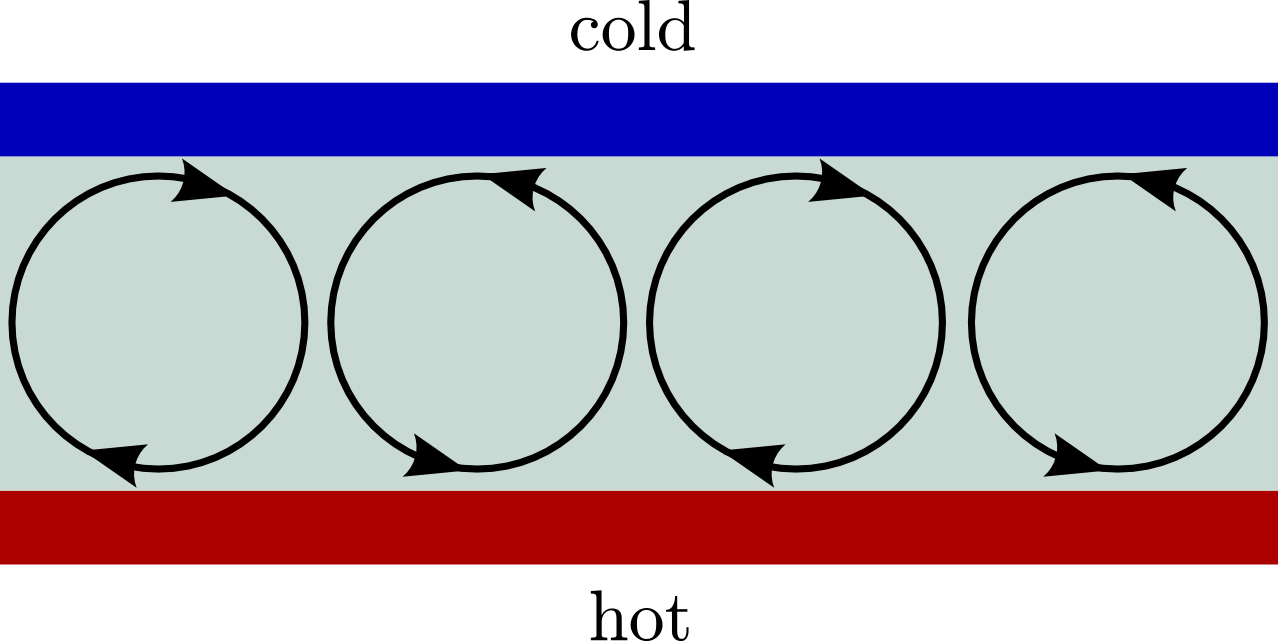
\includegraphics[width=0.5\linewidth]{hot-cold_5_.png}
	\caption{Convection Rolls: each circle represent a convection going between the top and bottom layers.}
	\label{fig:RBC_roll}
\end{figure}
This kind of motion can only maintain in a small area: If the path of the loop is too long, the frictions coming from the viscosity will damp the oscillation heavily, ending up with the deformation of the loop. Hence, for a complanate system, whose horizontal sizes are much larger than the vertical height, if being observed from a large scale under a suitable temperature difference, then the pattern on the horizontal plane seem to be an aggregation of many tiny convection cells~\footnote{The minimum volume containing a intact convectional loop is called a ``cell''.}, as it is shown in Figure~\ref{fig:RBC_cell}.\par
\begin{figure}[!ht]
	\centering
	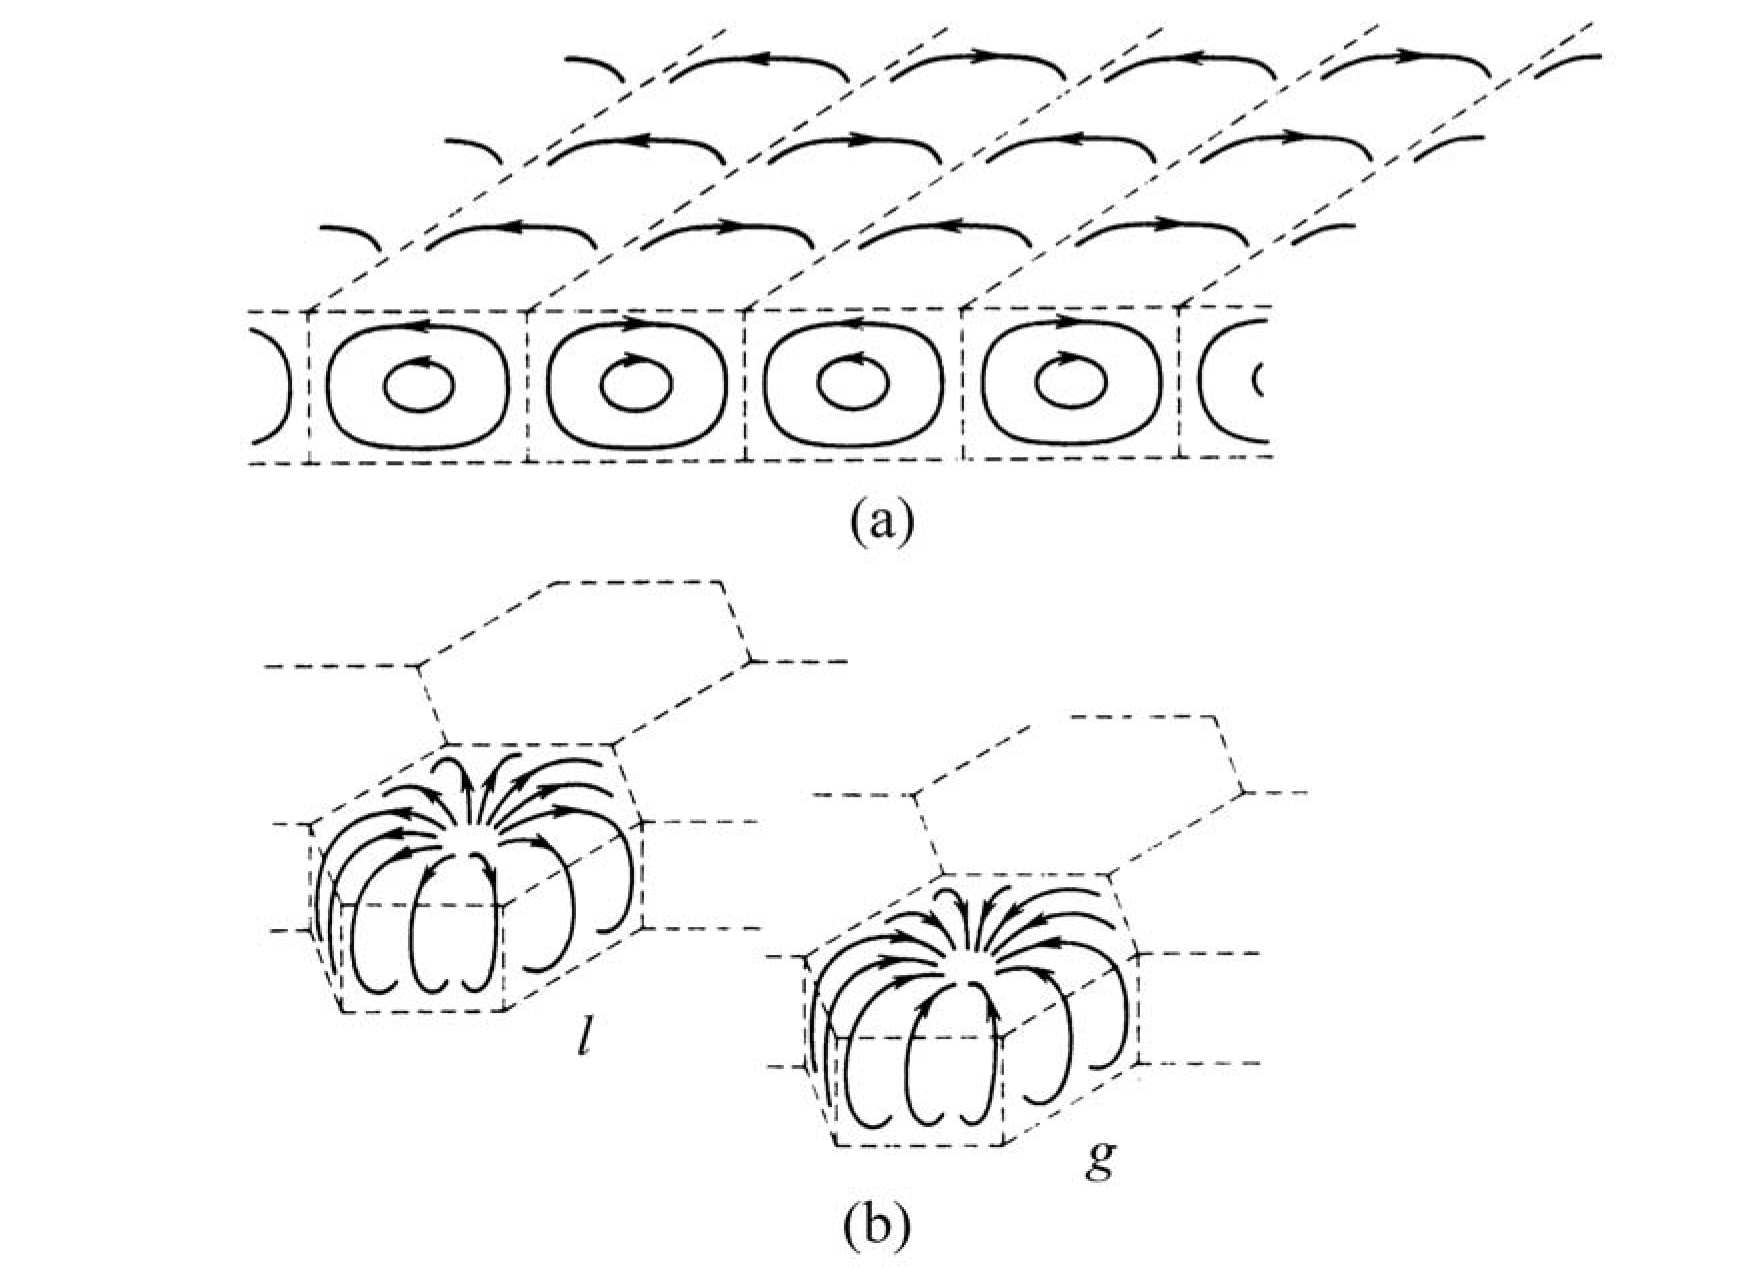
\includegraphics[width=0.6\linewidth]{Rayleigh_Benard_cells.png}
	\caption{Schematic of two types of convection cells for RBC: (a) rolls; (b) hexagonal convection cells of the l and g types.}
	\label{fig:RBC_cell}
\end{figure}
Convection cells are the fundamental elements of RBC. Two typical types of them are rolls and hexagonal. If the system
is with low temperature difference, then only few kinds of motions is allowed in the cell. These permitted motions are
identifies as normal modes determined by the boundary conditions. The normal modes analyze is to find out the possible normal modes of a system.\par
And convection can persistently transport heat from bottom to top, whose efficiency is considered to be useful. The way
to get it is based on the normal modes analyze, who is thought to be stony. In this report, we established systemically models for the convection occurring under different boundary conditions, and calculated the Nusselt Number, defined as the transporting ratio of the heat flux .\par 
The boundary conditions at the top and bottom layers are classified into two classes: boundary conditions for velocity field, and for thermal field. Each of the types has two cases: free surface without tangential stresses or rigid surface without slips, for velocity fields, prescribed temperature or prescribed heat flux, for thermal field. The combination of them will give four cases:
\begin{center}
\parbox[c]{0.9\linewidth}{
\begin{enumerate}
	\item free surface for velocity field and prescribed temperature for thermal field;
	\item free surface for velocity field and prescribed heat flux for thermal field;
	\item rigid surface for velocity field and prescribed temperature for thermal field;
	\item rigid surface for velocity field and prescribed heat flux for thermal field.
\end{enumerate}
}
\end{center}\par
Saltzman derived a group of nonlinear equations from Naiver-Stokes equation of RBC. And by substituting Fourier modes
into them, a numerical solution for case (a) was achieved. Lorenz simplified them to a dynamic system and discovered
chaotic behaviors. On the other hand, Chandrasekhar and Hurle has already characterized the normal modes for rigid boundaries of RBC, we apply them in approach of Saltzman to derive a dynamical system of Lorenz type for other three cases. Then, its dynamics can be analyzed.\par
As is well known to all, a state of a fluid system needs at least three quantities to represent. They are the three
components of the velocity \(u\left(x,y,z,t\right)\), \(v\left(x,y,z,t\right)\), \(w\left(x,y,z,t\right)\) along three
directions \(x\),\(y\),\(z\) correspondingly, the density distribution \(\rho\left(x,y,z,t\right)\) and the temperature
profile \(T\left(x,y,z,t\right)\). In addition, the height \(H\) and temperature difference \(\Delta T_0\) between the
layers and the viscosity \(\nu\), heat transparency \(\kappa\), heat expansion coefficient \(\alpha\) are also required. They can be combined into two dimensionless numbers: Prandtl Number \(\sigma=\nu/\kappa\) and Rayleigh number \(R=g\alpha H^3 \Delta T_0/\left(\kappa\nu\right)\) whose importance would be further discussed in below.\par
The situation we are interested in is not the extremely turbulent system so that the temperature difference \(\Delta T_0\) should be assumed not too high, which represents the motion won't go far away from the static state. Under this limits, the Boussinesq approximation can be introduced which has been precisely defined by the following sentence:
\begin{center}
	\parbox[c]{0.9\linewidth}{\textit{``In fluid dynamics, the \textbf{Boussinesq approximation} (pronounced, named for Joseph Valentin Boussinesq) is used in the field of buoyancy-driven flow (also known as natural convection). It ignores density differences except where they appear in terms multiplied by g, the acceleration due to gravity. The essence of the Boussinesq approximation is that the difference in inertia is negligible but gravity is sufficiently strong to make the specific weight appreciably different between the two fluids. Sound waves are impossible/neglected when the Boussinesq approximation is used since sound waves move via density variations.''}}
\end{center}
With the help of it, the transit from static to turbulent is simplified to a group of linear equations which can be analytically solved to obtain the normal modes.\par
The report is organized as follow: we first introduce the works of Saltzman and Lorenz in Chapter 2, to see how Lorenz model founded. Then we characterise the normal modes of other three cases in Chapter 3. \par
